%% Requires compilation with XeLaTeX or LuaLaTeX
\documentclass[10pt,xcolor={table,dvipsnames},t]{beamer}
%\documentclass[compress]{beamer}
\usetheme{diapo}
\usepackage{amsmath}
\usepackage[bottom]{footmisc}
\usepackage{multirow}
\usepackage[francais]{babel}

\title[Lorenz]{Application de la méthode para-real à la simulation d'EDP dans Feel++}
\subtitle{Présentation 1}
\author[name]{LECOURTIER Frédérique}
\institute{\large Université de Strasbourg}
\date{\today}

\begin{document}
	
	\begin{frame}
		\titlepage
	\end{frame}

	\AtBeginSection[]{
		\begin{frame}
			\vfill
			\centering
			\begin{beamercolorbox}[sep=5pt,shadow=true,rounded=true]{subtitle}
				\usebeamerfont{title}\insertsectionhead\par%
			\end{beamercolorbox}
			\vfill
		\end{frame}
	}

	\begin{frame}{Résultats actuels}
		Algorithme semble fonctionner.
		$$\sigma=10, \quad b=\frac{8}{3}, \quad r=28, \quad X_0=(5,5,5),$$ 
		$$t_0=0, \quad T=2, \quad \Delta t_G=0.1, \quad \Delta t_F=0.01$$
		\begin{figure}
			\centering
			\begin{minipage}{0.48\linewidth}
				\centering
				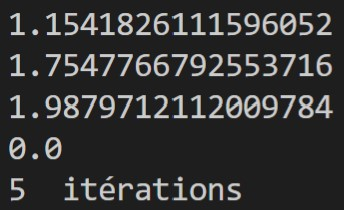
\includegraphics[width=0.5\linewidth]{images/erreur_python.jpg}
			\end{minipage}
			\begin{minipage}{0.48\linewidth}
				\centering
				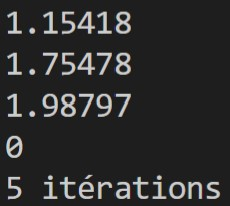
\includegraphics[width=0.35\linewidth]{images/erreur_cpp.jpg}
			\end{minipage}
			\caption{Erreurs entre chaque itération pour l'algorithme en Python et l'algorithme en C++ (pour les mêmes paramètres)}
		\end{figure}
	\end{frame}

	\begin{frame}{Problèmes}
		
		\begin{enumerate}[\textbullet]
			\item Problème avec communication collective (Scatter) -> remplacée par un Send/Recv
			\item Segmentation fault pour la mise en commun des résultats entre les processus -> utilisation de valgrind ?
		\end{enumerate}
	\end{frame}

	\begin{frame}{Prochaines étapes}
		Pour l'algorithme en C++ :
		\begin{enumerate}[\textbullet]
			\item Réussir à mettre en commun les résultats entre les processus et afficher les solutions.
			\item Faire la même étude de convergence qu'en Python (pour vérifier que l'algorithme fonctionne correctement)
		\end{enumerate}
		\; \\
		Quand l'algorithme sera implémenté, deux étapes principales :
		\begin{enumerate}[\textbullet]
			\item Implémenter la résolution de l'équation de Laplace en C++ avec Feel++
			\item Implémenter la résolution de l'équation de la chaleur en C++ avec Feel++
		\end{enumerate}
	\end{frame}


\end{document}